%!TEX TS-program = xelatex 
%!TEX encoding = UTF-8 Unicode
%
%  my_title
%
%  Created by David Perez on march 2010.
%  Copyright (c) David Perez 2010. All rights reserved.
%

% -*- Mode:TeX -*-



%% The documentclass options along with the pagestyle can be used to generate
%% a technical report, a draft copy, or a regular thesis.  You may need to
%% re-specify the pagestyle after you \include  cover.tex.  For more
%% information, see the first few lines of mitthesis.cls. 

%\documentclass[12pt,vi,twoside]{mitthesis}
%%
%%  If you want your thesis copyright to you instead of MIT, use the
%%  ``vi'' option, as above.
%%
%\documentclass[12pt,twoside,leftblank]{mitthesis}
%%
%% If you want blank pages before new chapters to be labelled ``This
%% Page Intentionally Left Blank'', use the ``leftblank'' option, as
%% above. 

%For the final thesis
\documentclass[12pt,vi]{mitthesis}
\pagestyle{plain} 

%for technical report
%\documentclass[12pt,vi,twoside]{mitthesis}
%\pagestyle{plain}

%for draft
%\documentclass[11pt,singlespace,draft]{mitthesis}
%\pagestyle{drafthead}


%%package for TODO lists, comments, annotations on pdf, with colors
%\usepackage[enable, spanish, colorinlistoftodos]{todonotes}
%%el comando de abajo hace el trabajo automaticamente identificando si es un
%%draft
%\usepackage[obeyDraft]{todonotes}
%%los posibles COLORES usados para \todo[color=green!40]{test12} son:
%%green, red, blue!20!white (para mezclar dos colores)
%%la UBICACION del comentario, en el borde o entre parrafos:
%%\todo[noline]{A note with no line ...} noline o line o inline
%%\missingfigure[figwidth=6cm]{Testing a long text string}

%\usepackage[pdfborder={0 0 0}]{hyperref}
\usepackage[colorinlistoftodos, textwidth=2.8cm, shadow]{todonotes}
\usepackage{amsmath}
\usepackage[displaymath, tightpage]{preview}



 
\usepackage{lgrind}

%% in case I include .eps versions of all figures for those w/o pdftex
%\usepackage{ifpdf}
%\ifpdf
%\usepackage[pdftex]{graphicx}
%\else
\usepackage{graphicx} 
%\fi

\usepackage{amsmath,amssymb,amsfonts} % easily align arrays of equations
\usepackage{hyperref} % hyperlinks
\usepackage{subfig} % multi-part figures
\usepackage{pdfpages} % makes it easy to insert all those nsigmapi fits


% Feynman diagrams
\usepackage{feynmp}
\DeclareGraphicsRule{*}{mps}{*}{}


%%%%%%%%%%%%%%%%%%%%%%%%%%%%%%%%%%%%%%%%%%%%%%%%%%%%%%%%%%%%%%%%%%%%%%%%%%
%%%%Paquete usado para rotar la pagina,
%%%%encontrado en http://texblog.wordpress.com/2007/11/10/landscape-in-latex/
\usepackage{pdflscape}





%%%%%%%%%%%%%%%%%%%%%%%%%%%%%%%%%%%%%%%%%%%%%%%%%%%%%%%%%%%%%%%%%%%%%%%%%%
%%%%%%%%%%%%%%%%%%%%begin code formatting%%%%%%%%%%%%%%%%%%%%%%%%%%%%%%%%%
%paquete para agregar codigo fuente
%\usepackage{listings}
\usepackage{listings}
\usepackage{courier}
\lstset{
         basicstyle=\footnotesize\ttfamily, % Standardschrift
         %numbers=left,               % Ort der Zeilennummern
         numberstyle=\tiny,          % Stil der Zeilennummern
         %stepnumber=2,               % Abstand zwischen den Zeilennummern
         numbersep=5pt,              % Abstand der Nummern zum Text
         tabsize=2,                  % Groesse von Tabs
         extendedchars=true,         %
         breaklines=true,            % Zeilen werden Umgebrochen
         keywordstyle=\color{red},
                frame=b,         
 %        keywordstyle=[1]\textbf,    % Stil der Keywords
 %        keywordstyle=[2]\textbf,    %
 %        keywordstyle=[3]\textbf,    %
 %        keywordstyle=[4]\textbf,   \sqrt{\sqrt{}} %
         stringstyle=\color{white}\ttfamily, % Farbe der String
         showspaces=false,           % Leerzeichen anzeigen ?
         showtabs=false,             % Tabs anzeigen ?
         xleftmargin=17pt,
         framexleftmargin=17pt,
         framexrightmargin=5pt,
         framexbottommargin=4pt,
         %backgroundcolor=\color{lightgray},
         showstringspaces=false      % Leerzeichen in Strings anzeigen ?        
 }
 \lstloadlanguages{% Check Dokumentation for further languages ...
         %[Visual]Basic
         %Pascal
         %C
         %C++
         %XML
         %HTML
         Java
}
    %\DeclareCaptionFont{blue}{\color{blue}} 

  %\captionsetup[lstlisting]{singlelinecheck=false, labelfont={blue}, textfont={blue}}
\usepackage{caption}
\DeclareCaptionFont{white}{\color{white}}
\DeclareCaptionFormat{listing}{\colorbox[cmyk]{0.43, 0.35, 0.35,0.01}{\parbox{\textwidth}{\hspace{15pt}#1#2#3}}}
\captionsetup[lstlisting]{format=listing,labelfont=white,textfont=white, singlelinecheck=false, margin=0pt, font={bf,footnotesize}}

%%%%%%%%%%%%%%%%%%%%end code formatting%%%%%%%%%%%%%%%%%%%%%%%%%%%%%%%%%%%%%%%%
%%%%%%%%%%%%%%%%%%%%%%%%%%%%%%%%%%%%%%%%%%%%%%%%%%%%%%%%%%%%%%%%%%%%%%%%%%%%%%%

\begin{document}

\include{cover}

\pagestyle{plain}
\include{contents}
\begin{fmffile}{feynman-diagrams}




%\\.
%\\. 
%\\.
%\\.
%\todo[inline]{Agregar la secci\'on del cover}
%	Debo agregar una hoja donde indique que estos cap\'itulos son
%	el marco teorico de la investigaci\'on, dicho comando para
%	agregar la palabra parte A por ejemplo, sin numeraci\'on de 
%	paginas en esta, voy a encontrar en el formato de tesis 
%	de la universidad de washintong basado en la del MIT, 
%	dicho template esta en mis archivos de Google Docs



\chapter*{Annotations}

Auxiliary chapter (not is part of this document content).
En esta parte explico sobre la plataforma latex que utilizo, sobre la
sistematizaci\'on que utilizo para redactar este documento, por ejemplo, que
significan los comentarios que hago con el comando TODO, etc.

\section{Convenci\'on de colores para los comentarios hechos en este documento}
	Un comentario de color 
	\emph{NARANJADO}
	\todo{Ejemplo}   
	indica las cosas que me faltan hacer.\\

	Un comentario de color 
	\emph{VERDE CLARO}
	\todo[color=green!40]{green!40}
	indica en que parte de la norma IEC 61850 se est\'a utilizando la teor\'ia
	comentada. Indica la relaci\'on del contenido bibliogr\'afico de conceptos con
	la norma. 
	Un ejemplo de uso de este tipo de comentarios en mi trabajo:
	En redes, cuando hablo de un concepto, por ejemplo, \emph{network
	reliability}, eso se habla en la norma, en la parte IEC 61850-xx, entonces yo
	indico en el comentario de que ese concepto se menciona en la tesis. 
	Esto es \'util para mi pues me sirve para justificar por que inclu\'i la 
	descripci\'on de alg\'un concepto en el trabajo, principalmente en el marco
	te\'orico, que utilizar\'e para describir todos los conocimientos necesarios
	para abordar la norma (por ejemplo: Redes, Programaci\'on orientada a
	objetos, UML).\\
	
	Los colores en \emph{LILA}
	\todo[inline, color=blue!50!red!50]{color=blue!50!red!50}
	indican peque\~nas variaciones de palabras que podr\'ia hacer pero no son de
	alta prioridad ni obligatorias de corregir (a mi punto de vista), pero
	la modificaci\'on de las partes comentadas mejorar\'ia la redacci\'on del
	texto, o bien explican por que hice esas mejoras o ubique, redacte, 
	o modifique de esa 	manera un determinado parrafo.
	

\section{Im\'agenes por agregar al trabajo}
	Por convenci\'on, utilizar\'e la siguiente imagen
	\missingfigure[color=green!40]{prueba del comando de falta de figura}
	para indicar de que est\'a faltando incluir la imagen en este lugar. Durante
	el proceso de redacci\'on se ir\'a agregando el contenido faltante




%%Agrega la lista de cosas (comentarios) que hay que hacer
\listoftodos



\chapter{Work Research Overview}

%\include{chapters/sample}
\section{Introduction}
For comming\ldots
%\section{Introduction}

Energy worldwide is at least a seven trillion dollar
a year business and expanding. Energy profoundly affects 
our economy, society, and environment \cite{Dukert:2009ab}, 
then, they are a continously researching about new technologies 
and standards in the electrical power systems, in areas such as 
information automation, related cyber security and data 
transfer performance through Smart Grids.

La energ\'ia en todo el mundo mueve por lo menos 7 billones de 
d\'olares anuales, y es un negocio en expansi\'on. Por ello, la 
energ\'ia afecta profundamente nuestra econom\'ia, sociedad y 
entorno \cite{Dukert2009}, debido a esto, existe una constante 
investigaci\'on, y han surgido nuevas tecnolog\'ias y est\'andares 
en los sistemas de potencia, en \'areas como la automatizaci\'on 
y tratamiento de la informaci\'on, por dar unos ejemplos, con el
objetivo de mejorar el performance y la seguridad en el sistema 
de potencia, a trav\'es de redes inteligentes (Smart Grids).

In the lasts years,  the power systems automation over the world
uses microprocessors embedded devices 
\cite{Santoso:2000, Schwarz:2000mc} called
Intelligent Electronic Devices (IEDs) that suport 
network communication technologies with
the aim of to send or receive information from or to many sources
to monitoring, control and supervise the generation, transmission 
and distribution of the energy. 

En los \'ultimos a\~nos, la automatizaci\'on de sistemas de potencia 
en todo el mundo utiliza ampliamente dispositivos basados en uno o 
varios microprocesadores \cite{Santoso:2000, Schwarz:2000mc} integrados 
llamados Intelligent Electronic Devices (IEDs)  que utilizan 
tecnolog\'ias de redes de comunicaci\'on con el objetivo de enviar 
o recibir informaci\'on de o para varias fuentes con el objetivo 
de monitorear, controlar, y supervisar la generaci\'on, transmisi\'on 
y distribuci\'on de la energ\'ia
   \cite{McDonald:2007, IEEE:1997dic, Schwarz:2008wi}.

The information interchagebility between IEDs from diferent
vendors was coming complex, expensive, and sometimes 
impossible, then the industry 

\ldots\ldots\ldots

to adopt the IEC 61850 standard to achieve the interoperability, 
realiability and more quality for the information interchange 
of the Energy Management System (EMS).

\ldots\ldots\ldots aca debo colocar las siglas de EMS, ver como
arreglar este tema para que quede todo bien el tema de las siglas
  

El intercambio de informaci\'on entre IEDs de diferentes fabricantes 
se ha vuelto muy complejo, costoso, y a veces imposible, es por ello 
que la industria se ha puesto de acuerdo para adoptar el est\'andar 
IEC 61850 y as\'i conseguir interoperabilidad, confiabilidad y mayor 
calidad en el intercambio de informaci\'on dentro del Sistema de 
Gerenciamiento de Energ\'ia (EMS-Energy Management System). 

The IEC 61850 standard ``Comunication Networks and Systems in Substations" 
provide a support for sustainable interoperability between IEDs: 
information model, information interchange methods, communications 
protocols mappings and a Substation Configuration Language (SCL) 
for electrical energy systems (Generation, Transmission and Distribution) 
for hight, might and low voltage \cite{Schwarz2008}. 

La norma IEC 61850 ``Comunication Networks and Systems in Substations" 
provee un perfecto soporte para una interoperabilidad sustentable entre 
IEDs: modelado de la informaci\'on, m\'etodos para intercambio de la 
informaci\'on, mapeo a protocolos de comunicaci\'on, y un lenguaje de 
configuraci\'on de subestaciones (SCL) para sistemas el\'ectricos de 
energ\'ia (Generaci\'on, Transmisi\'on y Distribuci\'on para alta, 
media y baja tensi\'on) \cite{Schwarz2008}. 

Initially, the standard IEC 61850 focuses on substations, 
and now it are extended to 

\ldots\ldots\ldots satisfacer no se decir..

the totality of the 

La norma IEC 61850, en la actualidad, no se enfoca \'unicamente a 
subestaciones, tambi\'en es aplicable y extensible para satisfacer 
las necesidades de casi la totalidad de la cadena de suministro de 
energ\'ia, entre los cuales destacamos la protecci\'on de l\'ineas de 
transmisi\'on, plantas de energ\'ia e\'olica, distribuci\'on de 
energ\'ia y centrales hidroel\'ectricas, sistemas fotovoltaicos y 
coches el\'ectricos \cite{Schwarz2005, DER2009, German2009}. 

El modelado jer\'arquico de la informaci\'on a trav\'es de nodos 
l\'ogicos es una cuesti\'on clave. La agrupaci\'on correcta de los 
nodos l\'ogicos representan funciones o equipos utilizados en los 
sistemas de potencia. Cada nodo l\'ogico provee una lista de informaci\'on 
bien designada y organizada. Los objetos y servicios definidos en la parte 
IEC 61850-7-2 de la norma permiten el intercambio de esta 
informaci\'on \cite{TC572004}.

En julio del 2007 las extensiones de los nodos l\'ogicos a centrales 
hidroel\'ectricas han sido aprobadas, publicadas y est\'an listas 
para su uso, en el apartado IEC 61850-7-4-10: 
\emph{Hydroelectric Power Plants - Communication for monitoring and control}; 
agregando 60 nodos l\'ogicos y 350 \emph{Data Objects} a la serie 
IEC 61850 \cite{IEC61850TC57, Schwarz2008b}.

Este trabajo consiste en la aplicaci\'on de la norma IEC 61850, 
en especial del modelado de nodos l\'ogicos definidos en la parte 
7-4-10 Hydro Power Plants y de los objetos y servicios de comunicaci\'on 
para la automatizaci\'on de una unidad generadora t\'ipica de Itaipu, 
y proponer al TC57 (International Electrotechnical Commission, Technical 
Committee 57) la complementaci\'on o extensi\'on de nodos l\'ogicos de 
la norma que actualmente son insuficientes para las unidades generadoras 
de Itaipu. Como estudio de caso, se modelar\'an los nodos l\'ogicos y 
servicios de comunicaci\'on necesarios para el regulador de velocidad de 
la unidad generadora. Este trabajo de investigaci\'on se basa en el \'item 
del documento ``Proposta de Temas para Monografias de 
Especializa\c c\~ao - Automa\c c\~ao, Controle e Supervis\~ao do 
Processo el\'etrico Baseado na Norma  IEC 61850 -  A-4 - Automa\c c\~ao 
de Unidades Geradoras - Modelagem Completa da Unidade Geradora" de la 
Itaipu Binacional, redactado por Marcos Fonseca Mendes, Antonio Sertich 
Koehler, Ladislao Aranda Arriola, funcionarios de la Itaipu Binacional. 

\section{Aim of this Research}
For comming\ldots

\section{Research Methodologies and Techniques}
Blah blah blah
\section{Originality of this Research}
Blah blah blah
\section{Organization of this Research Document}
This text is organized as follows:
For comming\ldots

\todo{traducir al ingles - organizacion de la tesis}

\begin{itemize}
  \item Chapter 1: revisi�n de la tesis 
  \item Chapter 2: \ldots
\end{itemize}

\todo[inline]{
		\emph{Cap�tulo: }hacer una revisi�n de la tesis
		
		\emph{capitulo: } 	capitulo introductorio a la norma IEC 61850,
						al estilo de la parte 1 y la parte 7-1, sin 
						entrar en puntos muy tecnicos, solo para dar 
						una nocion de lo que trata la norma, 
						asi como los famosos powerpoints que te 
						presentan para la norma y de dan una 
						nocion super super breve sobre que trata 
						la norma.
		
		\emph{Cap�tulo: }	hablar sobre programaci�n orientada 
						a objetos, uml y xml
						demasiado bien va a caer comenzar con
						este cap�tulo, dado que mi tema trata
						sobre modelado de objetos.
		
		\emph{Cap�tulo: } 	hablar sobre subestaciones, lo b�sico 
				para poder entender la norma. 
		
		\emph{Cap�tulo: } 		hablar sobre la automatizaci�n de usinas
				(basado en la tesis brasilera que me paso el Ing. Aranda)
		
		\emph{Cap�tulo: } 	hablar sobre redes, de absolutamente todos
				los conceptos necesarios.
		
		\emph{Cap�tulo: }	se puede estandarizar a UML las notaciones
				y explicaciones de arquitecturas que
				explica la norma. Posible contribucion: utilizar 
				OCL para mejorar la especificacion.
		
		\emph{Cap�tulo: }	hablar sobre la turbina itaip�
		
		\emph{Cap�tulo: }	hablar sobre la norma en si.
				(esto se puede subdividir otra vez
				en m�s cap�tulos especializados si es
				necesario)
		
		\emph{Cap�tulo: } 	se puede hablar sobre las funciones 
				de automatizaci�n aplicadas a la turbina 
				(o al regulador directamente) \\
		
		y los siguientes cap�tulos\ldots veremos despu�s\ldots
		tambien es probable de que varios de estos futuros 
		capitulos se fusionen en uno.
		
		
}


\todo[inline, color=blue!50!red!50]{hay capitulos que 
ya tengo bien aprendido, pero aun no escribi, en las 
vacaciones de invierno voy a escribir bien sobre redes
y las demas teorias basicas de automatizacion. Por 
el momento, he creado mapas mentales que apareceran 
en los capitulos inconclusos que ya tengo aprendido
pero solo me falta escribir. Para que pueda escribir, 
esos capitulos con un buen nivel tecnico voy a 
apoyarme en papers de varias asociaciones, principalmente
el de la IEEE. Aun no estoy pudiendo suscribirme y 
desde la CAPES no se accede, apenas pueda me suscribire 
y escribire esos capitulos. Siempre mi material 
principal es la norma en si, y en base a eso ya
tengo varios capitulos en mente (aprendidos 
pero por documentar) o ya escritos.}


 

\chapter{Introduction to the IEC 61850 series}



The IEC 61850 series defines de communications between 
intelligent electronic devices (IEDs) in the substation 
and the related system requirements.




For comming\ldots  

List of the IEC 61850 parts considered 
in this work: \todo{o por considerar} \\
IEC61850-1:2003 	\cite{IEC61850-1:2003} \\
IEC61850-2:2003		\cite{IEC61850-2:2003} \\
IEC61850-3:2002		\cite{IEC61850-3:2002} \\
IEC61850-4:2002		\cite{IEC61850-4:2002} \\
IEC61850-5:2003		\cite{IEC61850-5:2003} \\
IEC61850-6:2004		\cite{IEC61850-6:2004}  \\
IEC61850-7-1:2003	\cite{IEC61850-7-1:2003} \\
IEC61850-7-2:2003	\cite{IEC61850-7-2:2003} \\
IEC61850-7-3:2003	\cite{IEC61850-7-3:2003} \\
IEC61850-7-4:2003	\cite{IEC61850-7-4:2003} \\
IEC61850-7-410:2007	\cite{IEC61850-7-410:2007} \\
IEC61850-7-420:2009	\cite{IEC61850-7-420:2009} \\
IEC61850-7-430:200-X\cite{IEC61850-7-430:200-X} \\
IEC61850-7-5:2010	\cite{IEC61850-7-5:2010} \\
IEC61850-7-500:2010	\cite{IEC61850-7-500:2010} \\
IEC61850-7-510:2009	\cite{IEC61850-7-510:2009} \\
IEC61850-7-520:2010	\cite{IEC61850-7-520:2010} \\
IEC61850-7-10:2009	\cite{IEC61850-7-10:2009} \\
IEC61850-8-1:2004	\cite{IEC61850-8-1:2004} \\
IEC61850-9-1:2003	\cite{IEC61850-9-1:2003} \\
IEC61850-9-2:2004	\cite{IEC61850-9-2:2004} \\ 

\todo{debo arreglar las bibliografias del bibtex, 
no se estan viendo como se debe}

\begin{figure}
  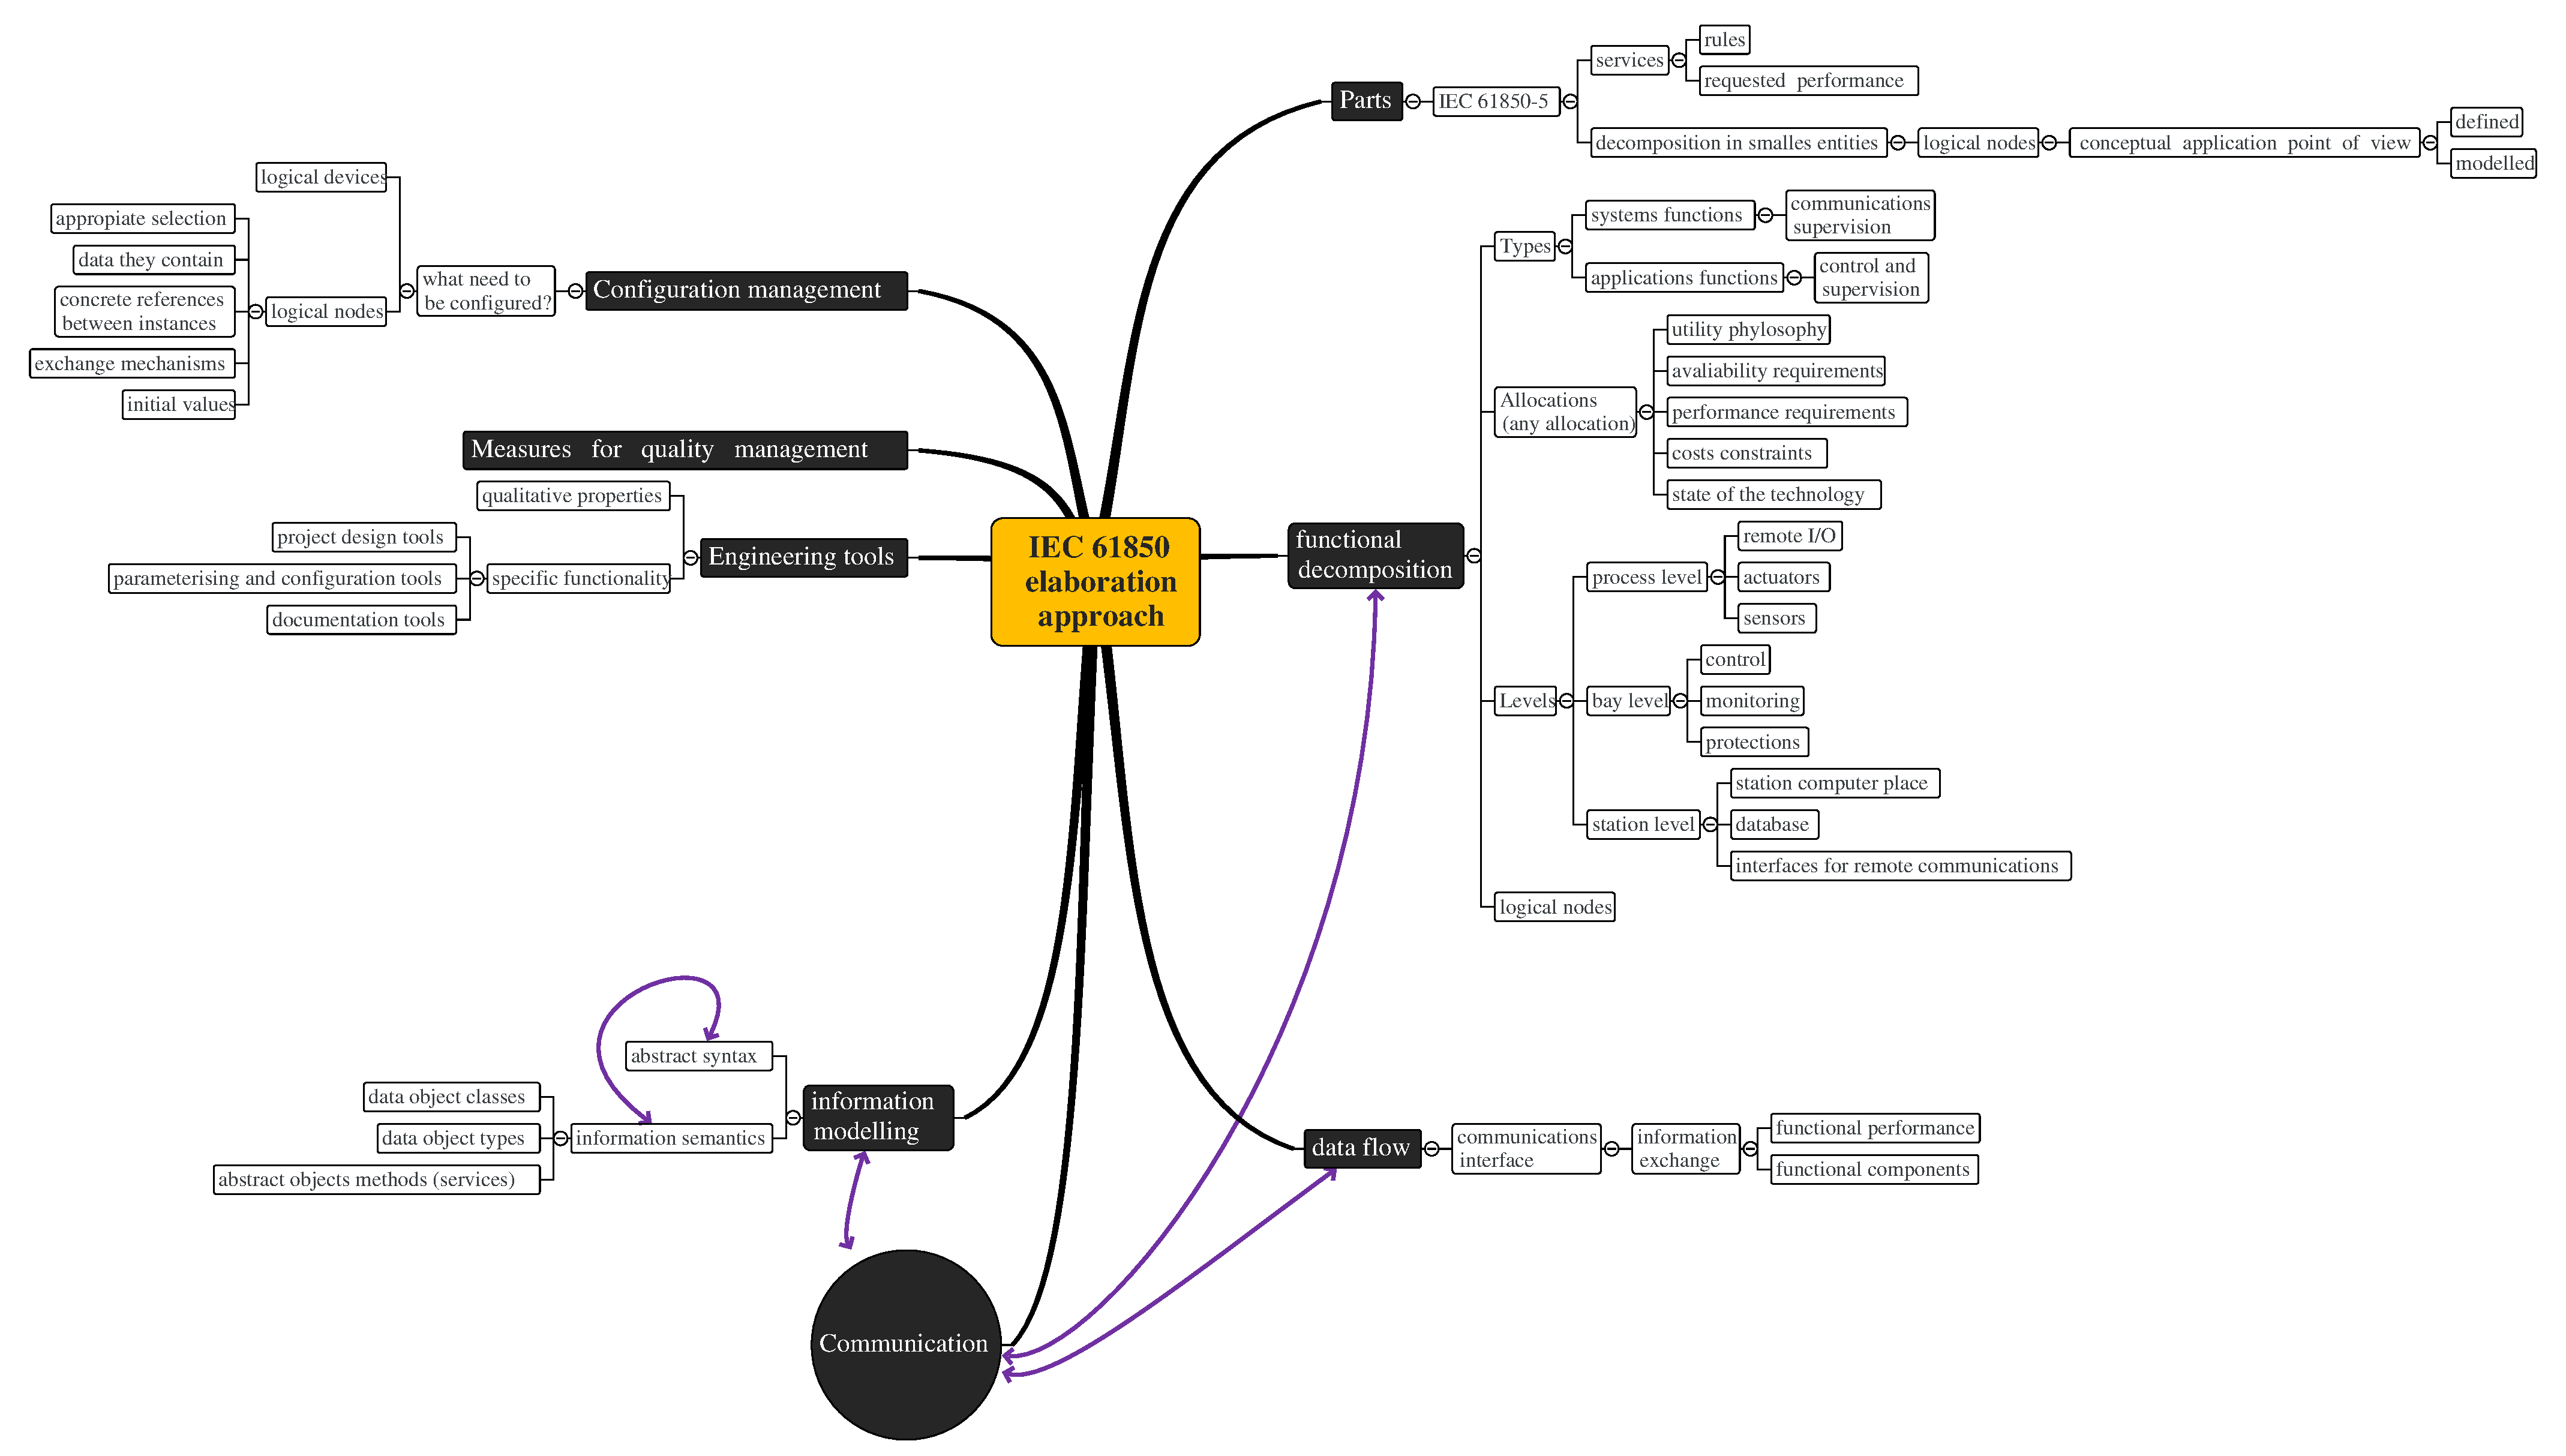
\includegraphics[width=1.0\textwidth]{appendices/IEC61850approach}
  \caption{Borrador - Esquema del futuro capitulo }
  \label{fig:lan-networks-topologies-fig3}
\end{figure}

\begin{figure}
  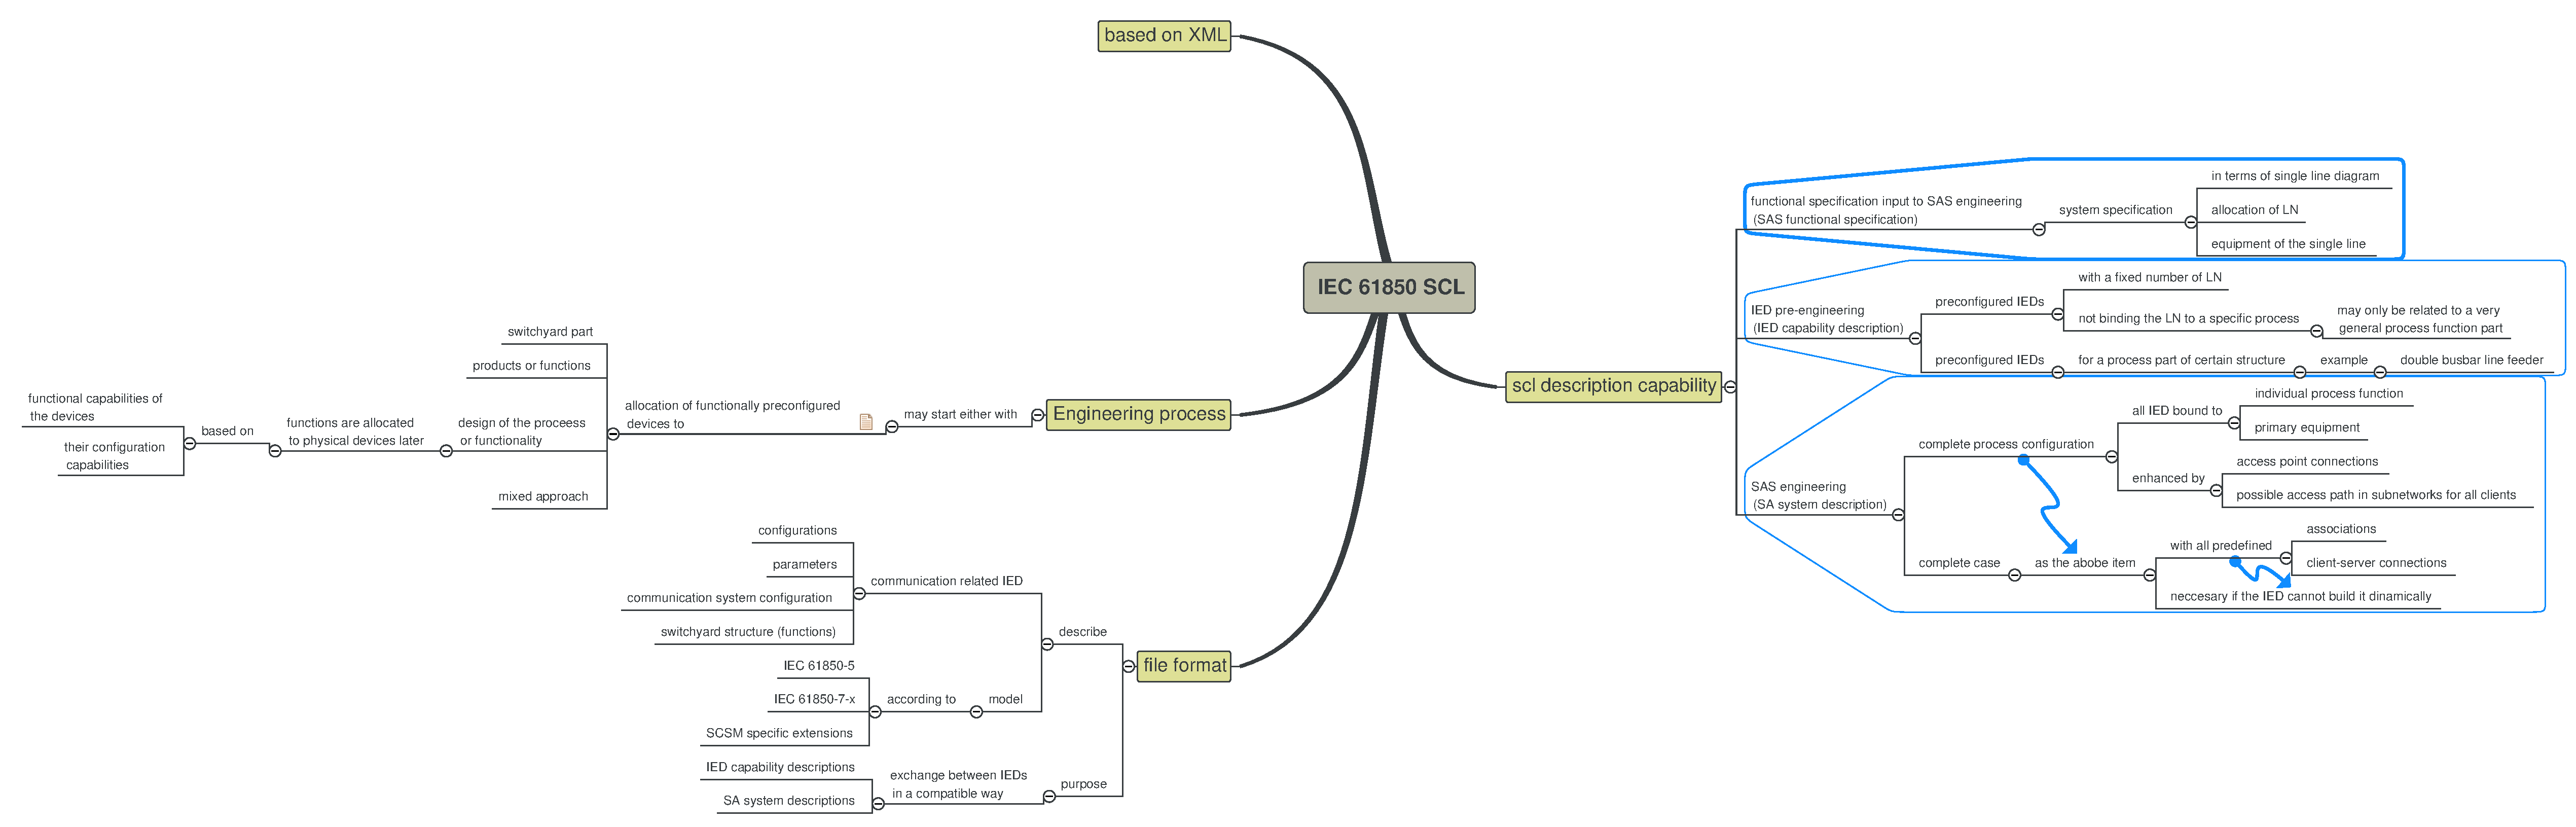
\includegraphics[width=1.0\textwidth]{appendices/IEC61850SCL}
  \caption{Borrador - Esquema del futuro capitulo }
  \label{fig:lan-networks-topologies-fig4}
\end{figure}

%%hello world!  first commit from linux! - this is a test

%%Este capítulo debe ser el primer tema técnico a tratar,
%%debido a que mi tema se trata al modelado de objetos 
%%y de servicios de comunicación (al final los servicios
%%de comunicación se modelan como objetos via xml)
%%y también la utilización de interfaces da una buena base
%%para entender las capas del modelo OSI: las interfaces
%%que posee cada capa para comunicarse con las otras
%%(servicios) son muy bien compreendidas una vez
%%tratada el tema de interfaces de OOP. Al final, 
%%este tema de interfaces es 
%%abstracción, tratada en ingeniería de software. Por 
%%ello, es un buen punto empezar desde aquí.

\chapter{Object-oriented system construction}

\section{Introduction}

This chapter describes the object-oriented programming (OPP) paradigm 
elements that will be used as the basis for the objects models 
in the IEC 61850 standard. The chapter does not describe 
general OPP principles, only focuses on 
the neccesary principles that will be used 
on the IEC 61850 engineering.
\section{Object Oriented systems}


%\todo[inline]{leer el paper de historia de poo, en la 2da pagina}
%\cite{Wegner:1987}

Many autors formulate precise 
definition of O-O paradigm 
\cite{Rentsch:1982} 
\cite{Pascoe:1986}
\cite{Nygaard:1986}
\cite{Madsen:1988}, 
and the definition of Lastly, Wegner 
\cite{Wegner:1987} has been 
the most widely 
accepted \cite{Capretz:2003}. Wegner defines 
the O-O paradigm in terms of objects, 
classes and inheritance.

\emph{
	``Objects are autonomous entities 
	that respond to messages or operations and share 
	a state. Classes classify objects by their common 
	operations. Inheritance serves to classify classes by 
	their shared behavior. Data abstraction hides the 
	representation of data and the implementation of 
	operations'' 
}\cite{Wegner:1987}. That is: 

object oriented = objects + classes + inheritance

In the next sections theses concepts are explained.

%This paradigm is useful to develop scalable, 
%consistent and reliable software systems 
%organizing the code to create objects. 
The O-O system programming metodology 
defines an approach to code organization 
for objects creation. 
The objects store the data and 
have their own behabiour with a 
particular information grouping 
by common functionality and common 
information structures. 
O-O systems benefits 
to bundle actions together, 
manage a few quantity of variables rather 
than multiples ones, 
organizing the 
common behavior together and 
structure programs in a way that
matches closely 
the real world \cite{Adobe:AS3man2008}. 


\section{Classes}

%%TODO: cite adobe book
%\input{chapters/ch-oop/classes-definitions}
A class is an abstract representation of an object. 
A class stores information about the types of data 
that an object can hold and the behaviors that an 
object can exhibit.

\subsection{Methods}
Methods are functions that are part of a class 
definition. Once an instance of the class is created, 
a method is bound to that instance.

	\subsubsection{Get and set accessor methods}
	Get and set accessor functions, also called getters 
	and setters, allow you to adhere to the programming principles of 
	information hiding and encapsulation while providing an 
	easy-to-use programming interface for the classes that you 
	create. Get and set functions allow you to keep your class 
	properties private to the class, but allow users of your class 
	to access those properties as if they were accessing a 
	class variable instead of calling a class method. 
	The advantage of this approach is that you can avoid 
	having two public-facing functions for each property 
	that allows both read and write access.
	
	\subsubsection{Constructor methods}
	Constructor methods, sometimes simply called constructors, 
	are functions that share the same name as the class in 
	which they are defined. Any code that you include in 
	a constructor method is executed whenever an instance of the 
	class is created with the  new  keyword.

\section{Objects}

The O-O program interaction is realized by 
objects invoking methods. 

\todo[inline]{falta completar}
\section{Diference betwen Classes and Objects}

They are a clear separation between 
class and object, and they are 
the most important concepts of O-O programming 
languages. \cite{Dahl:1970} 
%this separation was fist introduced by Simula 
%to simulate real-world applications. 

A class is a static off-line 
template to generate objects. 
A object is a runtime data 
or a group of datas 
according to the class. The objects are 
independend datas with 
its own behavior, and 
they are classified by the classes 
\todo{ESP:por las clases q la han generado}
which generated.


\section{The objects relationships}

\todo[inline, color=blue!50!red!50]{esto no va en la
seccion de objetos, pues antes necesite explicar 
la secci\'on \ref{sec:Diference-betwen-Classes-and-Objects} 
que trata sobre la diferencia entre objeto y clase. 
Esto es importante como una previa para esta seccion dado 
que las subsecciones a continuacion se presentan como 
clases pero describen las relaciones 
de los objetos. por eso es importante entender bien la 
diferencia primero. Esto es por el lector, para que 
le sea mas facil entender.}


	\subsection{Association}
		\todo{completar - association}
	
	\subsection{Aggregation}
		\todo{completar - aggregation}
		
	\subsection{Composition}
		\todo{completar - composition}
		
	\subsection{Other relationships}
		\todo[inline, color=blue!50!red!50]{por el momento 
		aca solo hay uno, por eso uso una subsubsection, 
		pero es altamente probable que coloque mas cosas
		si es que encuentro que son utilizados en la norma.}
		\subsubsection{Dependency}
			\todo{completar - dependency: la flechita del uml}

\section{Inheritance}

The inheritance can be used as a way to define new classes 
based in more general classes that have been 
defined previously, acquiring their characteristics.  
If a class \emph{CurrentTransformer} directly 
inherits from class \emph{Transformer} we say that 
\emph{Transformer} is the parent 
of \emph{CurrentTransformer} and 
\emph{CurrentTransformer} is the 
child of \emph{Transformer} \cite{Snyder:1986}. 
The UML representation is given in 
Figure \ref{fig:inheritance-fig}.



\begin{figure}
  \includegraphics[width=0.3\textwidth]{chapters/ch-oop/figures/inheritance}
  \caption{
  		Inheritance: \emph{Transformer} is the parent 
		of \emph{CurrentTransformer} and 
		\emph{CurrentTransformer} is the 
		child of \emph{Transformer}
		}
  \label{fig:inheritance-fig}
\end{figure}


\section{Information hidding and encapsulation}

	\subsection{Abstract data types}

Abstraction and information hidding form 
the foundation of all object-oriented 
development \cite{Levy:1984}. 
An abstraction is a simplified description, 
or specification, of a system that emphasizes 
some of the system's details or properties while
suppressing others \cite{Shaw:1984}.
Information hidding, as first promoted by Parnas,
\todo{explicar mas c/mis palabras} 
goes on to suggest that we should decompose 
systems based upon the principle of hidding 
design decisions about our 
abstractions \cite{Parnas:1979} \cite{Grady:1995}.

The abstraction and information hidding 
are very common in electrical equipments and 
mathematical representations of the 
electrical world. The 
models are abstracted 
and is possible to identify the object and 
operations that exist at each level of integrations 
Thus, 
when \todo[inline]{ver si las
palabras estan bien escritas
en este ejemplo} we work 
with phasors to represent a current, which 
leave just the static amplitude and phase
information. The time space are hidden with 
the purpose to manage the information 
at a more hight level, 
thereby skipping the trigonometric calculations 
derived from the time dependence of the sine wave, 
and the information are combined just algebraically, 
simplifying certain kinds of complex 
calculations.  \cite{Grady:1995}

%repetido!
%The abstraction  and information hidding are common 
%in our activities, we abstract the models by 
%identify the object and operations that exist 
%at each level of integration. Thus, when
%\todo[inline]{ver si las palabras estan 
%bien escritas en este ejemplo} 
%working a transformer, we consider the 
%taps, the current on the low and hight side, 
%the transformation relation \cite{Grady:1995}.

The use of abstract data types on a object oriented system 
help to a more precise and at the same time simple on the 
specification taking adventage of the information hidding 
provided by abstract 
data types. \cite{} \todo{aca debo citar mi paper sobre ACSI}





	\section{Intefaces}

%\input{chapters/ch-oop/blah blah blah}

	\section{Encapsulation}

\todo[inline]{Debo colocar algo aca}
	\subsection{Interfaces and implementation}

\todo[inline]{modificar, reelaborar con mis palabras}

Interfaces are based on the distinction between a 
methods interface and its implementation. A method’s interface 
includes all the information necessary to invoke that 
method, including the name of the method, all of its 
parameters, and its return type. A method’s 
implementation includes not only the interface 
information, but also the executable statements 
that carry out the method’s behavior. An 
interface definition contains only method 
interfaces, and any class that implements 
the interface is responsible for defining the 
method implementations. 
%%TODO: falta explicar más, enfocando desde 
%%el punto de vista de ingeniería de software
\cite[pp.~90-105]{Adobe:AS3man2008}

\todo[inline]{agregar aca lo que subraye
y resum� en
la segunda pagina del paper snyder:1986}	

\section{Events}



	\subsection{Event Dispatching}
	
	
	

\section{Exception handling}

%brevemente inspirado en este link
%http://www.allinterview.com/showanswers/59519.html
The exception is an unwanted and 
unexpeceted event which occours 
at runtime, and are caused by an unusual 
situation of the software that  
stop the normal secuence of  
software operations. 

When a exception event are 
dispatched by the system, 
the error could be handled 
by a specific modelled object 
if the software developer anticipated  
it as a posibility. 

The exception could be modelled 
with different handling stategies,     
\cite{MoonStallman:1983}
\cite{Dony:1988}
\cite{DonyC:1990}
\cite{Leavens:1991}
\todo[inline]{buscar mas papers de referencia 
			para colocar aqui por si alguien 
			tenga interes de profundizar en esto
			(buscar en la acm) }
%for example, could be represented 
%by classes of which 
%concrete exceptions would be some
%referenceable instances.  
for example, could be represented 
by classes specifically 
designed for this purpose of which 
concrete exceptions would be some
referenceable instances that 
handles the event of error. 

\begin{comment}
	\todo[inline]{leer la siguiente bibliografia:
	
	[MSW83] David Moon, Richard M. Stallman, and  Daniel Weinreb.  Lisp Machine 
	Manual  (fifth edition). Massachusetts Institute of Technology, Artificial Intelligence Laboratory, Cambridge, Mass., 
	January  1983.
	
	5.4 Exception Handling
	Hierarchies can also be used to classify 
	and organize exceptions in large 
	software systems. I think this was
	first done in the Flavors mechanism 
	of the Lisp Machine [MSW83]. Recent 
	papers on this topic include
	[Don88] [Don90].
	
	Extraido del paper: 
	introduction to the literature on O-O design, 
	programming and languages.
	Gary t. leavens
	}

esta tambien es una buena partida para saber los distintos
tipos de errores que no trato aqui por ser innecesarios
para la norma
http://www.sap-img.com/abap/difference-between-error-and-exception.htm
\end{comment}

\section{Serialization \todo[color=green!40]{61850, parte6, cl6.1, \textparagraph 3}
}
\todo[inline]{este parrafo a continuacion lo explique
con mis palabras, debo buscar algun paper que habla 
con un lenguaje mas tecnico para apoyar mi explicacion
y agregar las referencias correspondientes}
Serialization, or marshalling is the process of persist the object in memory 
or for transmission purpose, by creating a human readable 
archive that containts the object structure and datas 
in a saveable way. A object just exist at runtime, and 
it is serializad to be saved over the time or 
to be alternativatelly retransmited by the network 
to another host.
\section{Object oriented develoment approach}

The object-oriented development should 
follow the steps proposed by Aboott \cite{Abbott:1980}:  

\begin{itemize}
  \item Identify the objects and their attributes.
  \item Identify the operations suffered by and required
		of each object.
  \item Establish the visibility of each object in 
		relation to other objects.
  \item Establish the interface of each object.
  \item Implement each object.  
\end{itemize}



\chapter{Computer Networks}

\section{Introduction}

The purpose of this chapter is to provide the necessary background 
 to understand the concepts related to computer networks, 
focusing to explain the main concepts applied to the IEC 61850. 



\section{Transmission technologies}

Types of transmission technology:
\begin{itemize}
  \item Broadcast links.
  \item Point-to-point links.
\end{itemize}

Broadcast networks have a single communication channel 
that is shared by all the machines on the network. 
Short messages, called packets in certain contexts, 
sent by any machine are received by all the others. An 
address field within the packet specifies the intended 
recipient. Upon receiving a packet, a machine checks the 
address field. If the packet is intended for the receiving 
machine, that machine processes the packet; if the 
packet is intended for some other machine, 
it is just ignored. Some broadcast systems also 
support transmission to a subset of the machines, 
something known as multicasting \cite{Tanembaum:2003cn}. 

In contrast, point-to-point networks, sometimes 
called unicasting, consist of
many connections between individual pairs of machines. To go 
from the source to the destination, a packet on this 
type of network may have to first visit one or more 
intermediate machines. Often multiple routes, of 
different lengths, are possible, so finding good 
ones is important in point-to-point 
networks \cite{Tanembaum:2003cn}.



\section{Adressing and routing}

Each node must be able to say which of the other nodes on the 
network it wants to communicate with. This is done by assigning
an address to each node. An address is a byte string that identifies a node;
that is, the network can use a node’s address to distinguish it from the other
nodes connected to the network. When a source node wants the network to
deliver a message to a certain destination node, it specifies the address of
the destination node. If the sending and receiving nodes are not directly
connected, then the switches and routers of the network use this address to
decide how to forward the message toward the destination. The process of
determining systematically how to forward messages toward the destination node
based on its address is called routing \cite{PetersonDavie:2003}.

Adressing types: 

	\subsection{Unicast}
	The source node wants to send a message to a single destination node.
	
	\subsection{Broadcast}
	The source node want to \emph{broadcast} a message to all the 
	nodes on the network.
	
	\subsection{Multicast}
	The source node send a message to some subset of the 
	other nodes, but not all of them.
	

	
	
	

\section{Local Area Networks}
Local area networks, generally called LANs, are privately-owned 
networks within a single building or campus of 
up to a few kilometers in size. LANs are 
distinguished from other kinds of networks by three  
characteristics:
  
\begin{itemize}
  \item their size, 
  \item their transmission technology, and
  \item their topology.  
\end{itemize}

LANs are restricted in size,  which means that the 
worst-case transmission time is bounded and known in 
advance. Knowing this bound makes it possible to use 
certain kinds of designs that would not otherwise 
be possible. It also simplifies network management. 
LANs may use a transmission technology consisting 
of a ¿¿¿¿¿¿¿cable??????? to which all the machines 
are attached. Traditional  LANs  run  at  
speeds  of  10  Mbps  to  100 
Mbps, have low delay (microseconds or nanoseconds), 
and make very few errors. Newer LANs operate at up to 
10 Gbps. 

Various topologies are possible for broadcast LANs. 
Figure \ref{fig:lan-networks-topologies-fig} shows 
two of them. In a 
bus (i.e., a linear cable) network, 
at any instant at most one machine is the master 
and is allowed to transmit. All other machines are 
required to refrain from sending. An arbitration 
mechanism is needed to resolve conflicts when two or more 
machines want to transmit simultaneously. The 
arbitration mechanism may be centralized or 
distributed. IEEE 802.3, popularly called Ethernet, 
for example, is a bus-based broadcast network with 
decentralized control, usually operating at 10 Mbps 
to 10 Gbps. Computers on an Ethernet can transmit 
whenever they want to; if two or more packets collide, 
each computer just waits a random time and tries again later. 


\begin{figure}
  \includegraphics[width=1.0\textwidth]{chapters/ch-networks/figures/lan-networks-topologies}
  \caption{Two broadcast networks. (a) Bus. (b) Ring \cite{Tanembaum:2003cn}}
  \label{fig:lan-networks-topologies-fig}
\end{figure}

\section{Annotations}

Abcdef abcdef abcdef abcdef abcdef abcdef abcdef abcdef abcdef
\todo[size=\tiny]{test12 3test1 23tes t123}
abcdef abcdef abcdef abcdef abcdef abcdef abcdef abcdef abcdef
\todo[color=green!40]{test12 3test1 23tes t123} 
abcdef abcdef abcdef abcdef abcdef abcdef abcdef abcdef abcdef
\missingfigure{prueba del comando de falta de figura}
abcdef abcdef abcdef abcdef abcdef abcdef abcdef abcdef abcdef

\chapter{IEC 61850: Technical overview}

\section{Objects for distributed systems}

The effective distribution of Logical Nodes 
on diferents IEDs  
is a reality thanks to researches about 
the structure of distributed systems. More 
than 20 years ago emerged requirements 
for the object paradigm to suport the 
design and development of distributed systems.

Theses quotes were extracted from Jazayeri 
1988 research:

\emph{
``An object on one node can send a (multicast) message 
to several other objects \ldots''
} (MCAA) \todo{completar y ver si esta bien}

\emph{
`` \ldots The ability to group 
a set of objects and address them as one entity 
is important in many applications both from an 
efficiency point of view and from a program 
structuring point of view \ldots'' 
} (DO, DATA-SET, FCD, FCDA)\todo{completar y ver si esta bien}

\emph{
`` \ldots a final 
difference is that our objects are active and 
not reactive, in the sense that they can start 
up spontaneosly performing operations, not 
necessarily only in response to method invocations.
Such a facility is useful, for example, to allow objects 
to monitor the enviroment and change their behavior based 
on changes in the enviroment \ldots'' 
} (Some active objects 
are GOOSE, URCB and some passive object 
are \todo{completar y ver si esta bien})

\cite{Jazayeri:1988}.



\begin{figure}
  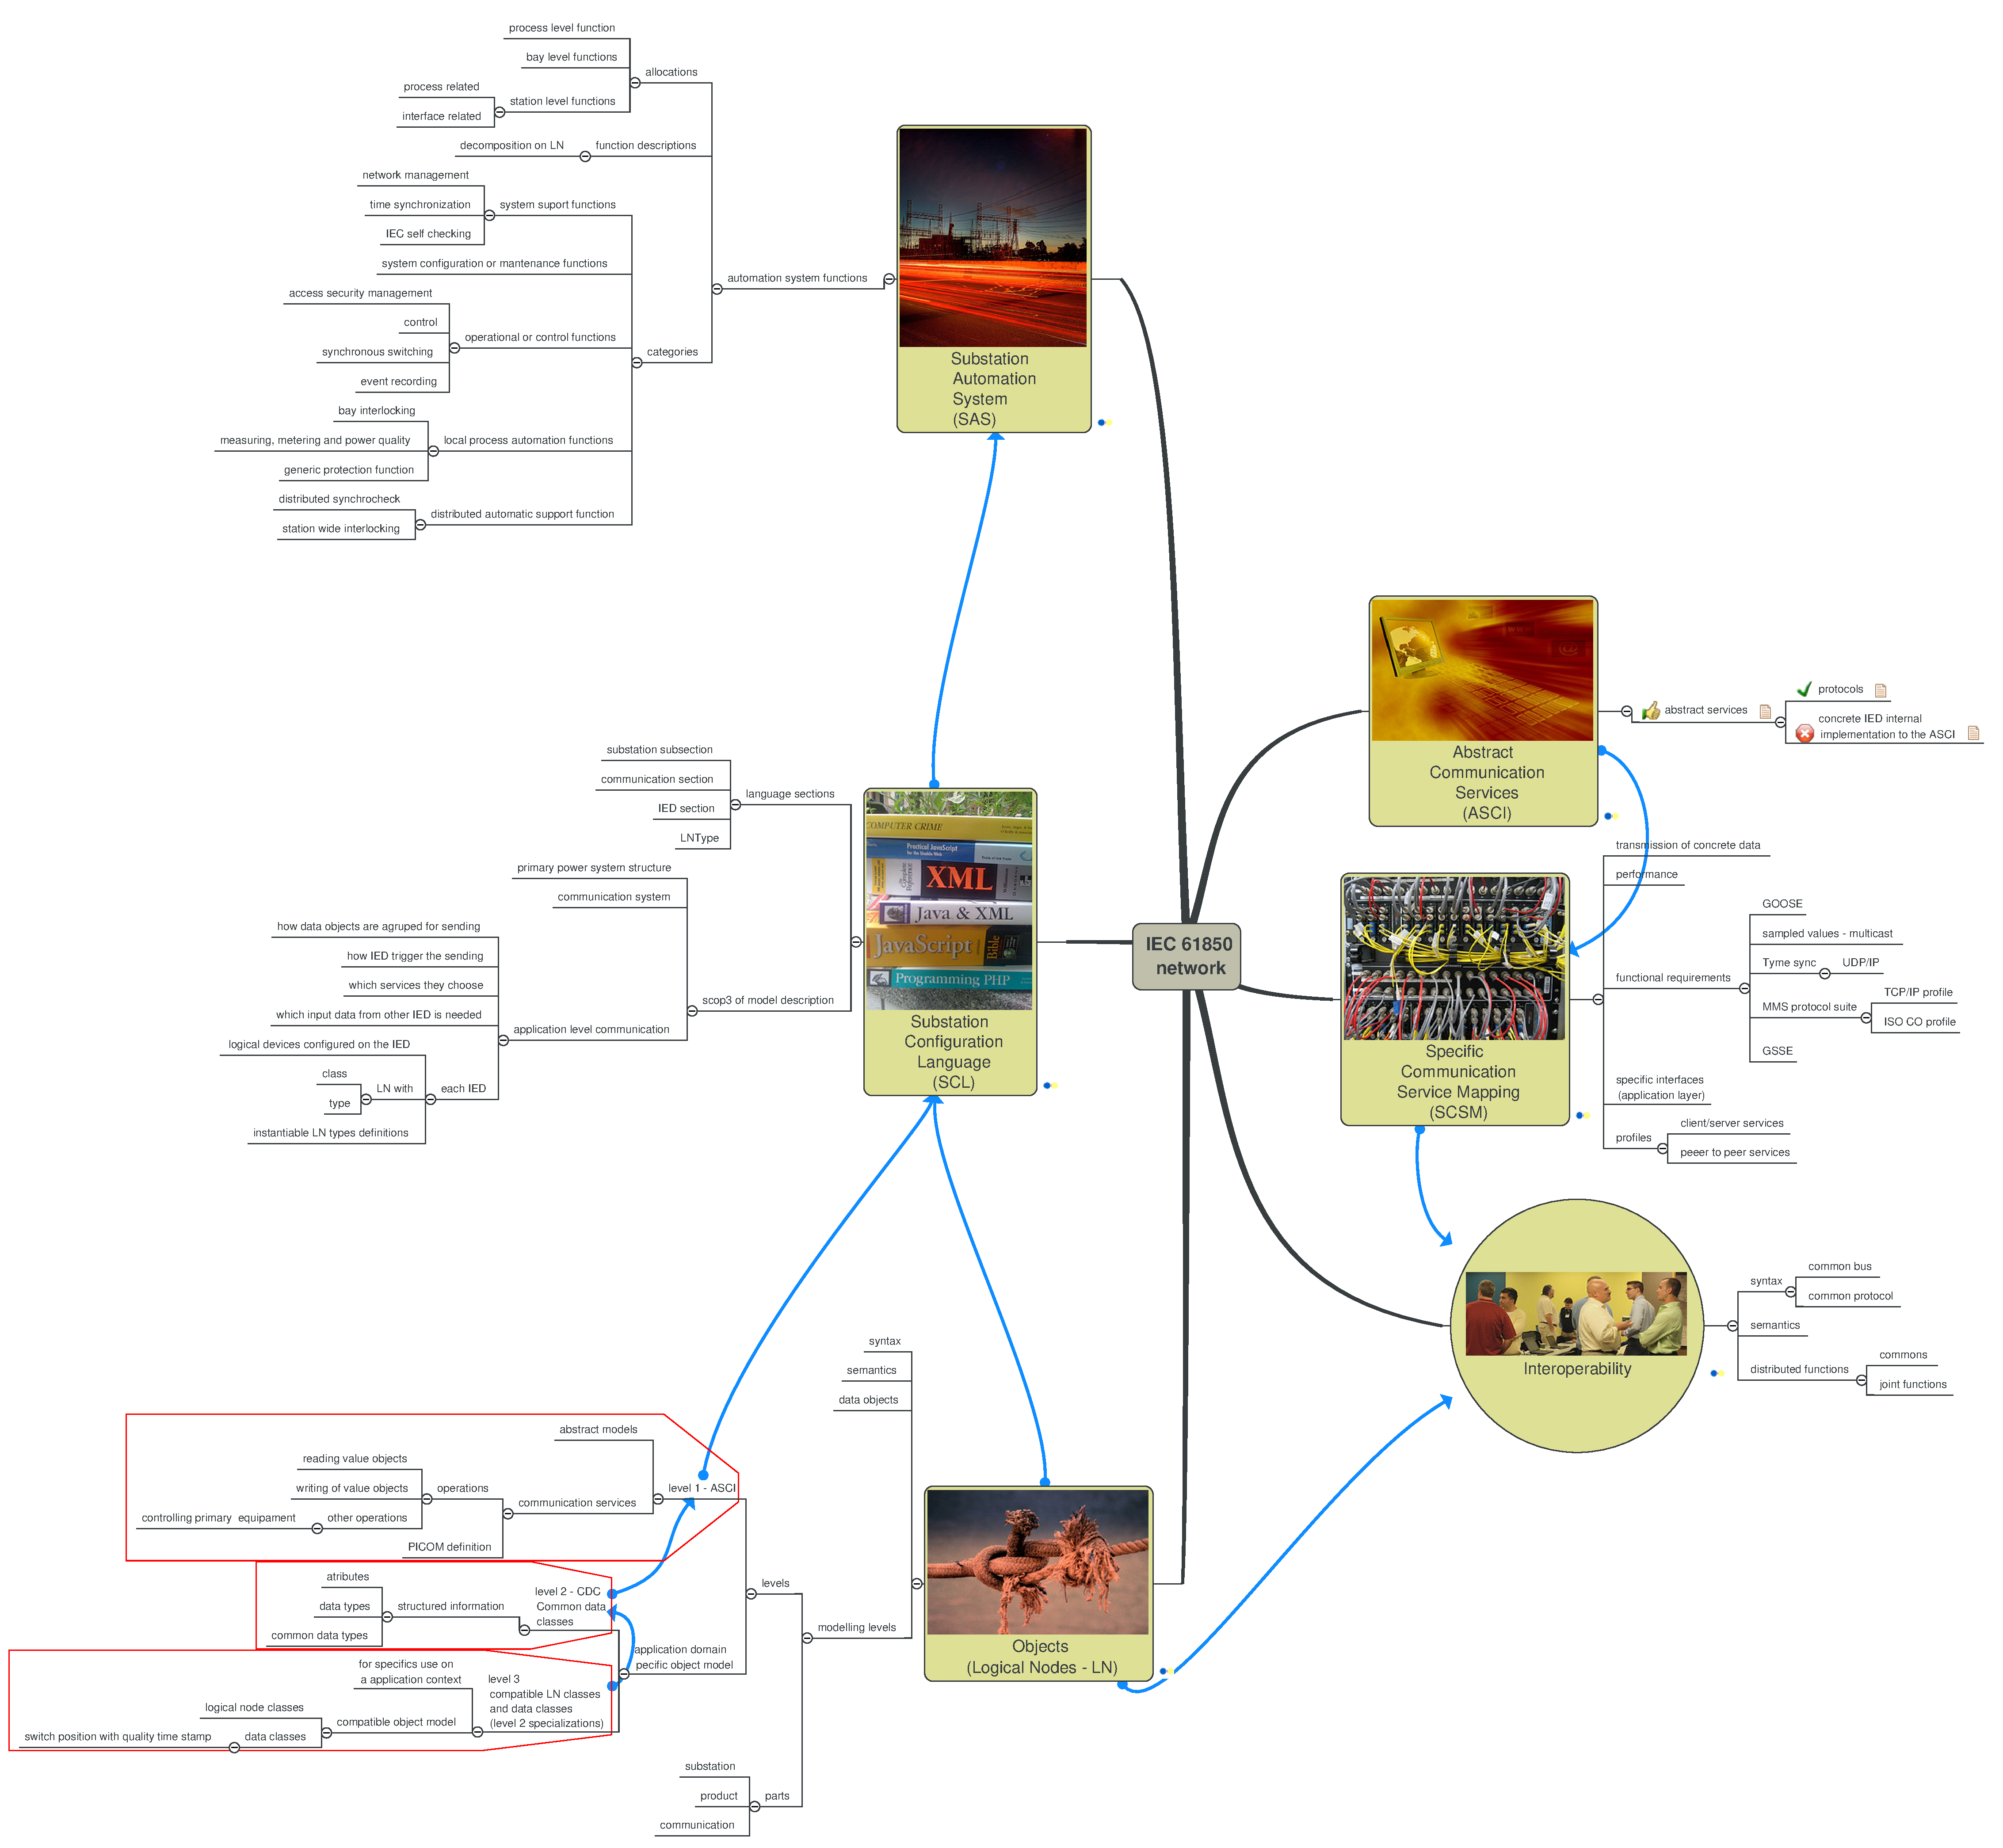
\includegraphics[width=1.0\textwidth]{appendices/IEC61850network}
  \caption{Borrador - Parte del esquema del futuro capitulo }
  \label{fig:lan-networks-topologies-fig1}
\end{figure}

\begin{landscape}
	\begin{figure}
	  \includegraphics[angle=-90, width=1.0\linewidth]{appendices/JavaPrinting}
	  \caption{Borrador - Parte del esquema del futuro capitulo }
	  \label{fig:lan-networks-topologies-fig2}
	\end{figure}
\end{landscape}
 



\chapter{Substation Configuration Language}

\section{Introduction}

The IEDs in conformance with the 
IEC 61850 allow a communication related 
configuration with 
a standarized description language 
called SCL, and they are specified 
in the part 6 of 
the IEC 61850 standard \cite{IEC61850-6:2004}.

This chapter describes the IEC 61850-6 \cite{IEC61850-6:2004} 
from a perspective of the defined model. This 
point of view will be useful for the 
nexts chapters where the SAS objects will be 
modelled in conformance with this standard.   

A Substation Configuration Language describes 
an instance of the SCL classes in a serialized form 
and standarized description of constraints and object structure. 
\todo[color=green!40]{61850, parte6, cl6.1, \textparagraph 3}

\todo{agregar mas cosas aca..}


\todo[inline]{en la breve introduccion del capitulo
debo explicar de que yo no mode\'e estas clases, 
sino que simplemente las estoy representando
de una manera conveniente para que sea entendible,
yo no invente nada aca, los graficos uml pertenecen
directamente al SCL.xsd definido en la norma,
yo simplemente represento los xsd en uml
para que sea mas facil explicar la estructura
y los constraints que exiran en el 
modelado de objetos basados en 
las clases uml descriptas en este capitulo}



\section{SCL engineering parts} \label{sec:SCL-engineering-parts}

The SCL description capability are 
an important \gls{SAS} engineering part, and may
start either with the SAS functional specification, 
\gls{IED} capability description or with the 
\gls{SAS} description. Theses steps 
are explained 
in the following subsections: 

\subsection{SAS functional specification}
The functional specification input to \gls{SAS} engineering 
consist in the system specification in terms of 
single line diagram, allocation of the \glspl{LN} 
and equipmets of the single line.

\subsection{IED capability description}
Another right name for this step is IED pre-engineering. 
In this step are described the IED capabilityes, for 
example, a IED with the double busbar line feeder function.

\subsection{SAS description}
This is part of the \gls{SAS} engineering, where the 
complete process configuration takes place: All IED 
are bounded to individual process functions and primary 
equipments, enhanced by access point connections and 
the access path in subnetworks for the clients.

A complete \gls{SAS} description provides 
all predefined associations and client-server connections 
(the \gls{IED} cannot built it automatically).

\todo[inline]{ver como puedo ir concatenando las ideas, hasta
desenvocar en este diagrama de secuencia}
A more detailed description are provided by this UML secuence diagram.

\begin{figure}
  \includegraphics[width=1.0\textwidth]{chapters/ch-scl/figures/SCL-development-process}
  \caption{SCL engineering process}
  \label{fig:SCL-development-process}
\end{figure}


\section{Tools}

The are tools used for the engineering steps 
mentioned in section \ref{sec:SCL-engineering-parts} 
and they are 


\section{SCL conformace}
%\section{SCL conformace in the IEC 61850 context}

The SCL files shall be validate with the 
\glspl{XSD} defined by the 
IEC 61850-6 \cite{IEC61850-6:2004} , and 
the IEDs shall handle theses SCL files 
in conformance with the specification.
The responsibilities listed below are 
defined by \cite[clause 5]{IEC61850-6:2004}. %paragraph 7

	\subsection{The IED responsability for SCL handling}
	\begin{itemize}
		\item 	The IED shall describe their capabilities by providing 
	 			the SCL file or it shall provide a external tool which 
	 			can generate the SCL file from the IED. 
	 	\item	The IED shall contain a alternative to setup the 
	 			communication: 
	 			
	 			\begin{itemize} 
                   \item Can use a system SCL file or 
                   \item can be accompained by a external 
                   		 tool which can import 
	 					 a two-party tool generated SCL file to the IED.
	 			\todo[inline]{al decir two party me 
	 			refiero a heramientas
	 			 de otras empresas, no se si se dice two-party 
	 			 o third-party.}
	 			 \end{itemize}
    \end{itemize}
 	 

\section{SCL object model}

\todo[inline]{en algun lado debo hablar de los conceptos
de SCL, que es, explicar de que es un lenguaje basado en xml, y 
que su estructura esta descripta en los XSDs definidos 
en la parte 6 de la norma}

As explained in section \ref{fig:pdf-SCL-uml-deept2} \todo{completar bien la referencia}, 
the SCL describes the SAS by modelling objects.
The standard IEC 61850-6 \cite{IEC61850-6:2004} object model 
structure and constraints are described in terms of the 
Schema Definition Language (XSD) \todo{abreviacion, corregir}.

The XSD of the SCL are structured as depicted 
in the figure \href{fig:pdf-SCL-uml-deept2}. 
Basically, it is composed by: 
\todo[color=green!40]{61850, parte6, cl6.1, \textparagraph 5}

\begin{itemize}
  \item The substation model: the object model of the primary power structure
  		(a instance of tSubstation) with their designations structured according to 
  		IEC 61346-1 \cite{IEC61346-1:1996}. 
  \item The communication model: the object model of the IED 
  		communication system configuration, 
  		i.e.,
  		the the networks, subnetworks, ports informations
  		\todo[color=green!40]{61850, parte6, cl6.1, \textparagraph 5},
  		the communication connection relations of IEDs to 
  		subnetworks, the routing for another subnetworks informations, 
  		and clocks configuration information and locations for 
  		time synchronisation (the gateways are not considered here, 
  		a gateway has to be modelled as another IED)
  		\todo[color=green!40]{61850, parte6, cl6.1, \textparagraph 8}.
  \item The product model: Contains the IEDs objects and their 
  		logical node implementations. 	
\end{itemize}

\todo[inline]{debo agregar aca la explicacion de los demas modelos
descriptos mediance los XSDs, pues esos tres 
items que menciona la norma son solo los mas
importantes, pero no da para entender y saber leer 
los archivos scl sabiendo solo eso. Los tres items mencionados arriba
son solo la base. Falta principalmente el DATypeTemplate
que corresponden a los objetos a serializar correspondientes 
a las instancias de las clases de la parte 7-x}

\begin{landscape}
	\begin{figure}
	  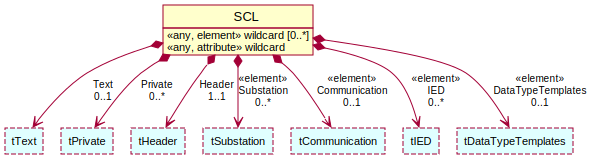
\includegraphics[angle=-90, width=1.0\linewidth]{chapters/ch-scl/figures/SCL-uml-Deept2}
	  \caption{SCL object model}  
	  \label{fig:pdf-SCL-uml-deept2}
	\end{figure}
\end{landscape}


\begin{landscape}
	\begin{figure}
	  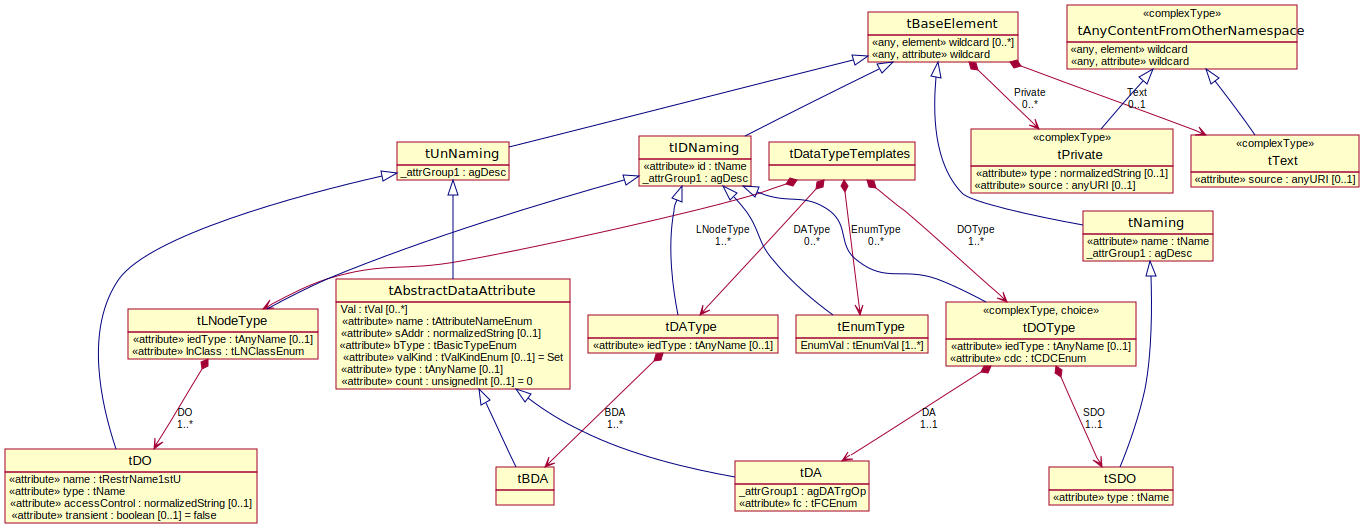
\includegraphics[angle=-90, width=1.0\linewidth]{chapters/ch-scl/figures/SCL-uml-DATypeTemplate-Deept2}
	  \caption{DAType object model template with heritance details}  
	  \label{fig:pdf-SCL-uml-DATypeTemplate-Deept2}
	\end{figure}
\end{landscape}

\begin{landscape}
	\begin{figure}
	  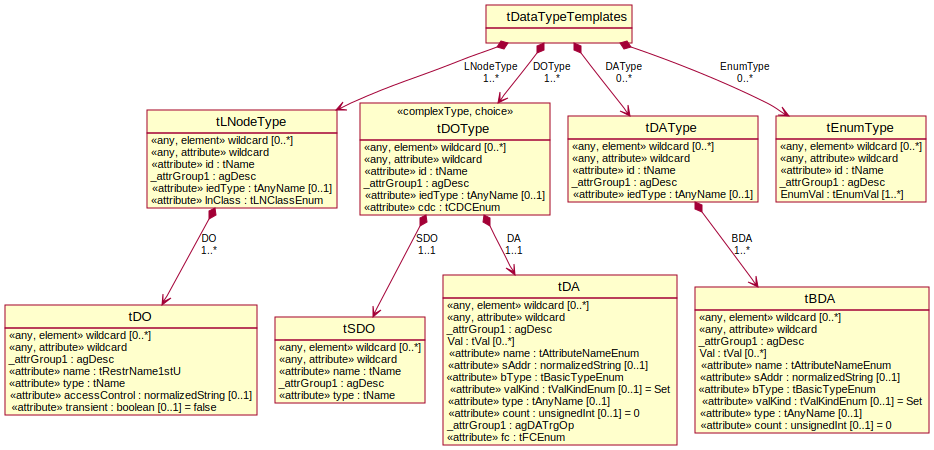
\includegraphics[angle=-90, width=1.0\linewidth]{chapters/ch-scl/figures/SCL-uml-DATypeTemplate-Deept2-inherited}
	  \caption{DAType object model template inherited}  
	  \label{fig:pdf-SCL-uml-DATypeTemplate-Deept2-inherited}
	\end{figure}
\end{landscape}

\begin{landscape}
	\begin{figure}
	  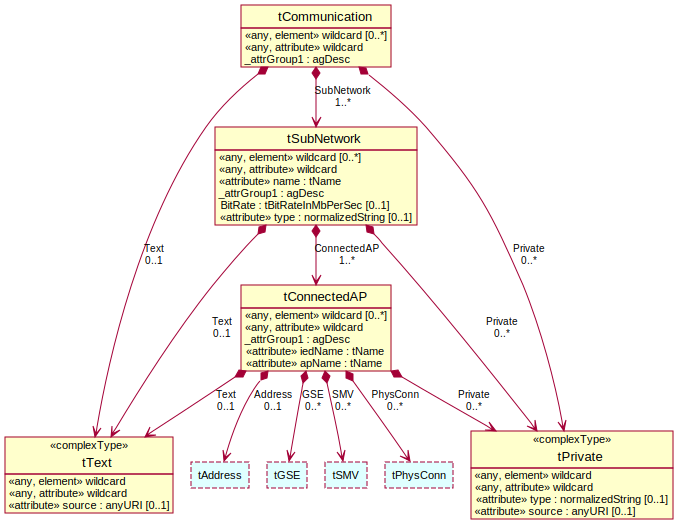
\includegraphics[angle=-90, width=1.0\linewidth]{chapters/ch-scl/figures/SCL-uml-communication-Deept3}
	  \caption{SCL Communication object model}  
	  \label{fig:pdf-SCL-uml-communication-Deept3}
	\end{figure}
\end{landscape}

\todo[inline]{podria convenir cambiar la palabra object model por class diagram
en todos estos graficos}

\todo[inline]{a este le valta
expandir la clase correspondiente hasta que muestre el transformador }
\begin{figure}
  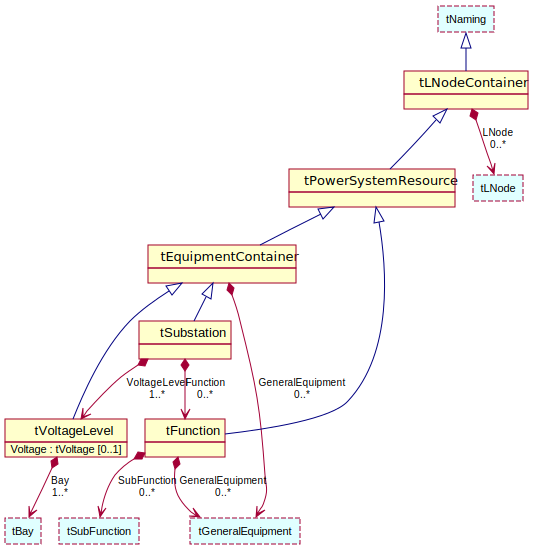
\includegraphics[width=1.0\linewidth]{chapters/ch-scl/figures/SCL-uml-substation-Deept2}
  \caption{SCL Substation object model with heritance 
  details  } 
  \label{fig:pdf-SCL-uml-substation-Deept2}
\end{figure}


\todo[inline]{a este le valta
  expandir la clase correspondiente hasta que muestre el transformador }
\begin{figure}
  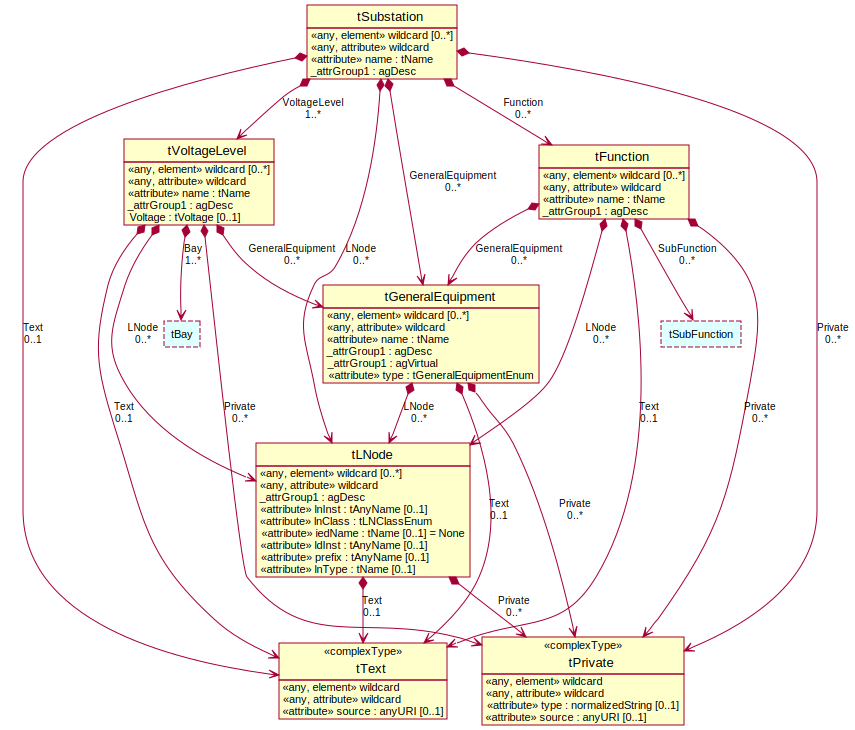
\includegraphics[width=1.0\linewidth]{chapters/ch-scl/figures/SCL-uml-substation-Deept2-inherited}
  \caption{SCL Substation object model inherited  }
  \label{fig:pdf-SCL-uml-substation-Deept2-inherited}
\end{figure}

The UML of the 
figure \ref{fig:SCL-uml-Resumen} 
is a resume of
the SCL model, where is evident the 
key importance of the Logical Node for  
the information topology description (see 
the composition of the Substation 
class). The Logical Node is  
the transition object to 
connect the diferent structures of the SAS 
\todo[color=green!40]{61850, parte6, cl6.1, \textparagraph 9} 
that are defined by IEC 61341-1 \cite{IEC61346-1:1996}.


\begin{landscape}

\begin{figure}
  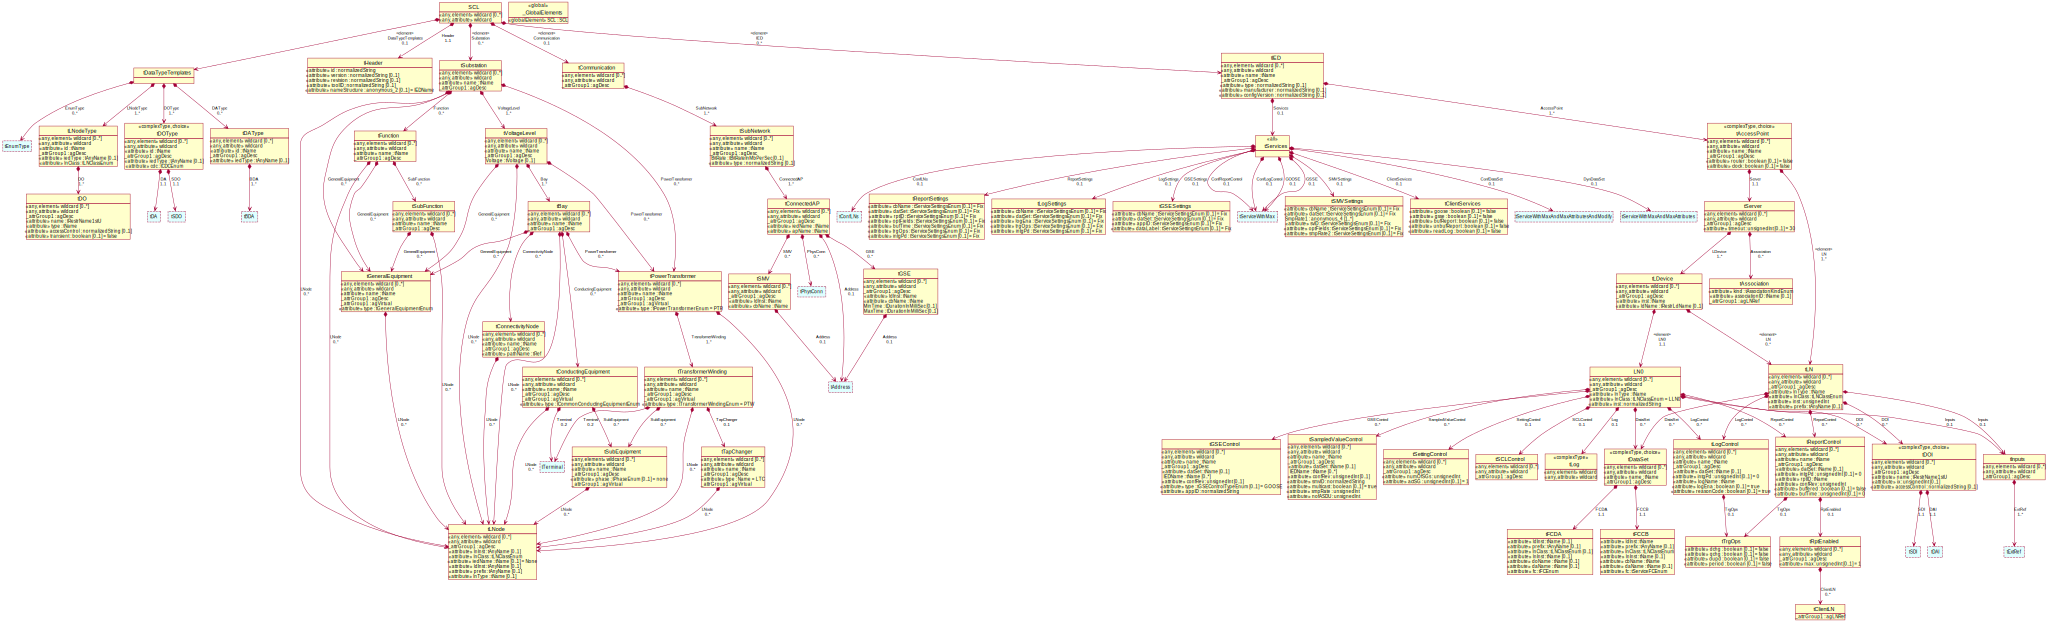
\includegraphics[angle=-90,
  width=1.0\linewidth]{chapters/ch-scl/figures/SCL-uml-Resumen-inherited}
  \caption{Resume of SCL shema represented by a UML class diagram}
  \label{fig:SCL-uml-Resumen}
\end{figure}
\end{landscape}

\section{SCL sections}

\begin{itemize}
  \item The \gls{SSD} contains a header and a substation sections.
  \item The \gls{ICD} contains a header, IED, and optionally a Substation
  template sections.
  \item The \gls{SCD} contains a header, substation, communication, multiple
  IEDs and multiple Data Type Templates.
  \item The CID \todo{agregarle los acronimos} contains a header, IEDs and
  their values, one instance of communication, and optionally a substation section. 
\end{itemize}

\section{A practical object modelling case with SCL}




\subsection{Complete SSD}
%scl-Example-T1-1-SSD-complete.xml
\lstinputlisting[label=code:TCTR_v1java,
caption=Example
of SSD]{chapters/ch-scl/source/scl/scl-Example-T1-1-SSD-complete.xml}

\\




 
%\include{ch1-theory}
%\include{ch2-experiment}
%\include{ch3-reconstruction}
%\include{ch4-analysis}
%\include{ch5-results}
%\include{ch6-conclusions}


\end{fmffile}
 \appendix
% \include{appendices/appa}
%% \include{appendices/appb}
\begin{singlespace}



%esta es la bibliografia standard de la IEEE
\bibliographystyle{IEEEtran}
\bibliography{IEEEabrv,bibliography/myIEEEbibliography}
%\bibliographystyle{plain}
%\bibliography{bibliography/myIEEEbibliography}

%\bibliography{main}
%\bibliographystyle{plain}
\end{singlespace}
\end{document}

